	
	\subsection*{1.}
	\begin{center}
		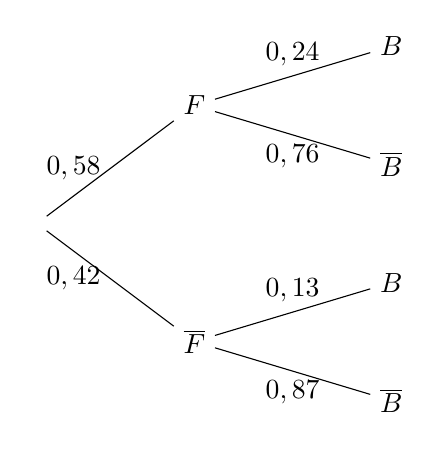
\begin{tikzpicture}
			[level 1/.style={level distance=2cm,
				sibling distance=3cm},
			level 2/.style={level distance=2.5cm,
				sibling distance=1.5cm}]
			\node {} [grow'=right]
			child {node {$F$}
				child {node {$B$}
					edge from parent node[above] {$0,24$}
				}
				child {node {$\overline B$}
					edge from parent node[below] {$0,76$}
				}
				edge from parent node[left] {$0,58$}
			}
			child {node {$\overline F$}
				child {node {$B$}
					edge from parent node[above] {$0,13$}
				}
				child {node {$\overline B$}
					edge from parent node[below] {$0,87$}
				}
				edge from parent node[left ] {$0,42$}
			}
			;
		\end{tikzpicture}
	\end{center}
	
	\subsection*{2.}
	On a :
	\[
	p(F \cap B) = p(F) \times p(B|F) = 0,58 \times 0,24 = 0,1392.
	\]
	
	\subsection*{3.}
	D'après la loi des probabilités totales :
	\[
	p(B) = p(B \cap F) + p(B \cap \overline{F}).
	\]
	Or,
	\[
	p(B \cap \overline{F}) = p(\overline{F} \cap B) = p(\overline{F}) \times p_{\overline{F}}(B) = 0,42 \times 0,13 = 0,0546.
	\]
	Donc,
	\[
	p(B) = 0,1392 + 0,0546 = 0,1938.
	\]
	
	\subsection*{4.a}
	\(X = 65\) correspond à l'évènement \(F \cap B\) de probabilité \(0,1392\);
	
	\(X = 40\) correspond à l'évènement \(F \cap \overline{B}\) de probabilité \(0,58 - 0,1392 = 0,4408\);
	
	\(X = 85\) correspond à l'évènement \(\overline{F} \cap \overline{B}\) de probabilité \(0,0546\);
	
	\(X = 60\) correspond à l'évènement \(\overline{F} \cap \overline{B}\) de probabilité \(0,42 - 0,0546 = 0,3654\).
	
	D'où le tableau :
	
	\[
	\begin{array}{|c|c|c|c|c|}
		\hline
		X = x_i & 40 & 60 & 65 & 85 \\
		\hline
		p(X = x_i) & 0,4408 & 0,3654 & 0,1392 & 0,0546 \\
		\hline
	\end{array}
	\]
	
	\subsection*{4.b}
	On a :
	\[
	E(X) = 40 \times 0,4408 + 60 \times 0,3654 + 65 \times 0,1392 + 85 \times 0,0546 = 53,245 \approx 53,25.
	\]
	Sur un grand nombre de clients, la dépense moyenne par client sera de 53,25 €.
	
